%\documentclass[a4,semhelv,landscape]{seminar}
\documentclass[landscape]{slides}
%\documentclass[landscape,aspectratio=169]{slides}
%\documentclass[pdf, default, slideBW, nocolorBG]{prosper}
\usepackage[left=0.2cm,top=0.2cm,right=0.2cm,bottom=0.2cm,nohead,nofoot]{geometry}
%\def\everyslide{\sffamily}
%\usepackage{fullpage}
\usepackage{graphicx}
\usepackage[usenames]{color}
%\usepackage{color}
\usepackage{verbatim}
\usepackage{nopageno}
\usepackage{setspace}
%\usepackage{times}
% define some nice colors
\definecolor{myred}{rgb}{0.6,0,0}
\definecolor{myblue}{rgb}{0,0.2,0.4}
\definecolor{mygreen}{rgb}{0,0.5,0.0}
\definecolor{mypurple}{cmyk}{0.5,1.0,0.0,0.0}
\definecolor{myorange}{cmyk}{0.0,0.75,1.0,0.0}
%\color{myblue}

\begin{document}
%%%%%%%%%%%%%%%%%%%%%%%%%%%%%%%%%%%%%%%%%%%%%%%%%%%%%%%%%%%%%%%%%%%%
%Slide 0 - title
\begin{slide}
\begin{center}
\large{\textbf{Automated validation and annotation of \\ SARS-CoV-2 sequences for GenBank using VADR}}

\normalsize

Eric Nawrocki \\
Staff Scientist \\

\medskip

\medskip

\medskip

\medskip

\medskip

\small
\begin{tabular}{c}
%\\
Computational Biology Branch \\
%National Center for Biotechnology Information\\
National Center for Biotechnology Information\\
%National Institutes of Health\\
National Library of Medicine \\
\\
\end{tabular}

\vspace{0.1in}


\includegraphics[width=2.5in]{figs/NIH_NLM_ABRV_2C_4-white}

\includegraphics[width=2.5in]{figs/ncbi-logo}

\end{center}
\end{slide}
%%%%%%%%%%%%%%%%%%%%%%%%%%%%%%%%%%%%%%%%%%%%%%%%%%%%%%%%%%%%%%%%%%%%%%
\begin{slide}
\begin{center}
\large{\textbf{GenBank indexers handle incoming sequence submissions}}
\end{center}

\center{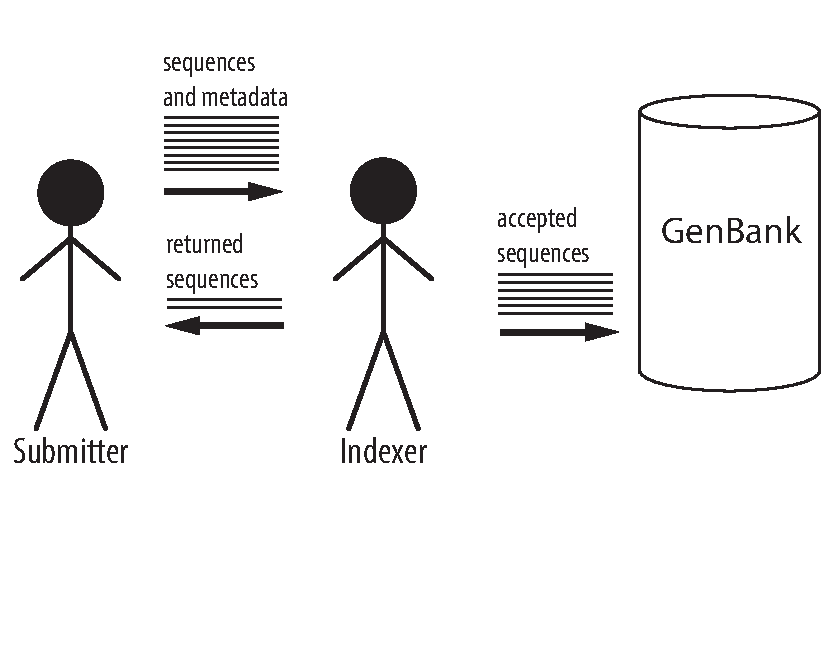
\includegraphics[width=9in]{figs/spheres-submission-schematic-1}}

\vfill
\end{slide}
%%%%%%%%%%%%%%%%%%%%%%%%%%%%%%%%%%%%%%%%%%%%%%%%%%%%%%%%%%%%%%%%%%%%%%
\begin{slide}
\begin{center}

\includegraphics[width=10in]{figs/vadr-title-paper}

\begin{itemize}
\item general tool for reference-based annotation of viral sequences
\item used for Norovirus and Dengue virus submissions since 2018
\item used for SARS-CoV-2 submissions since March 2020 
\end{itemize}

\vfill
\end{center}
\end{slide}
%%%%%%%%%%%%%%%%%%%%%%%%%%%%%%%%%%%%%%%%%%%%%%%%%%%%%%%%%%%%%%%%%%%%%%
\begin{slide}
\begin{center}
\large{\textbf{VADR assists GenBank indexers: \\ Each sequence \textcolor{green}{PASSes} or \textcolor{red}{FAILs}}}
\end{center}

\center{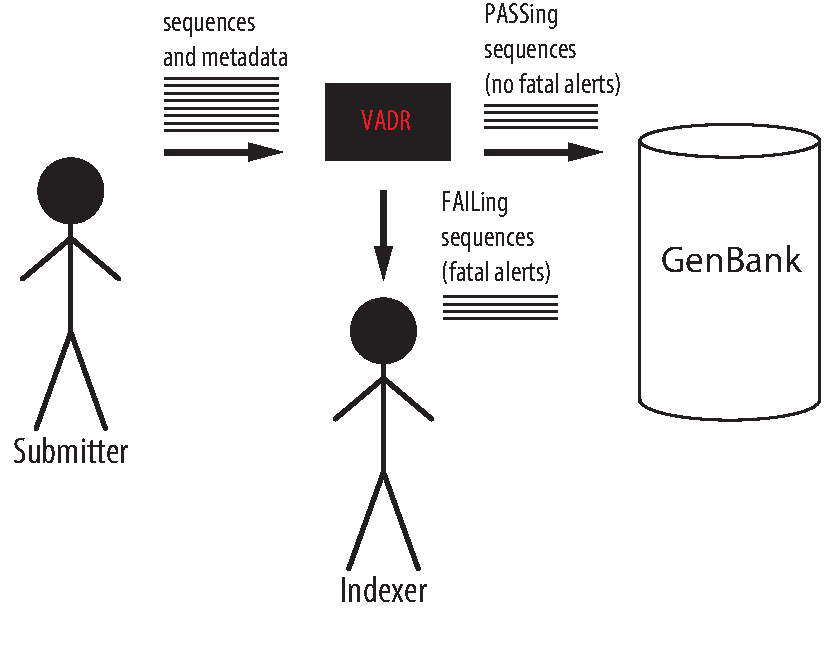
\includegraphics[width=9in]{figs/spheres-submission-schematic-2}}

\vfill
\end{slide}
%%%%%%%%%%%%%%%%%%%%%%%%%%%%%%%%%%%%%%%%%%%%%%%%%%%%%%%%%%%%%%%%%%%%%%
\begin{slide}
\begin{center}
\textbf{Indexers decide fate of some \textcolor{red}{FAILing} sequences\\ but some are sent directly back to submitter with error reports}
\end{center}

%\center{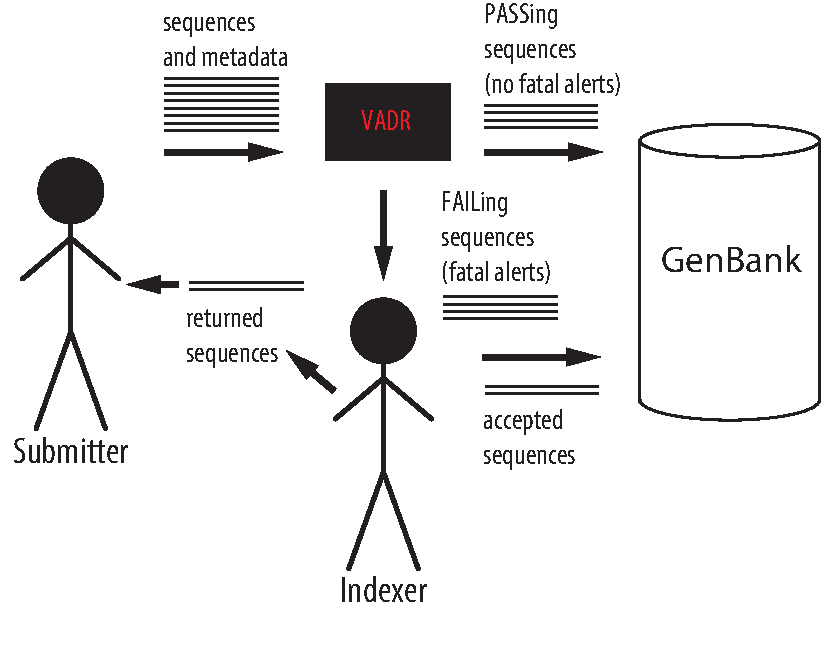
\includegraphics[width=9in]{figs/spheres-submission-schematic-3}}
\center{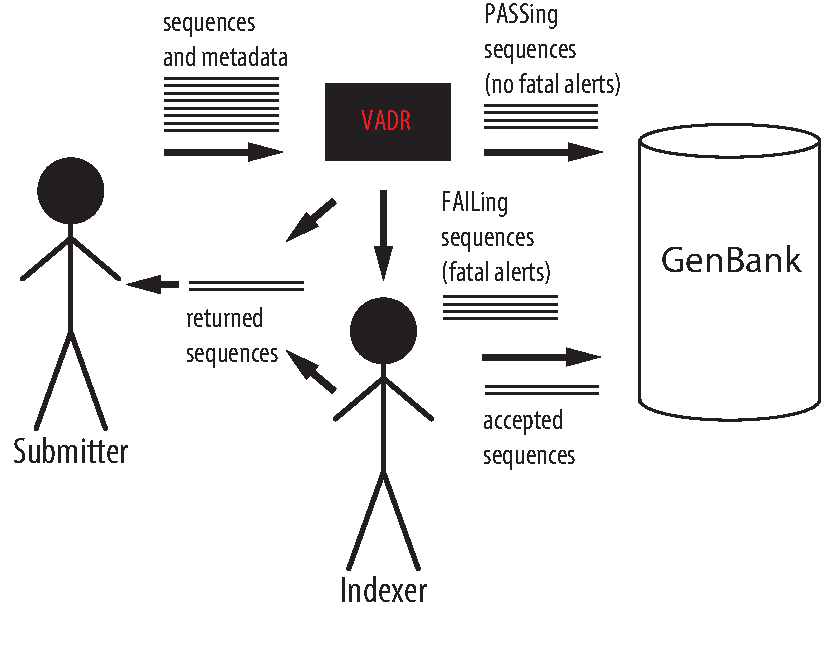
\includegraphics[width=9in]{figs/spheres-submission-schematic-4}}

\vfill
\end{slide}
%%%%%%%%%%%%%%%%%%%%%%%%%%%%%%%%%%%%%%%%%%%%%%%%%%%%%%%%%%%%%%%%%%%%%%
\begin{slide}
\begin{center}
%\textbf{\texttt{v-annotate.pl} annotates each sequence using its
\textbf{VADR proceeds over four stages to validate and annotate sequences}

\begin{itemize}
\item For each sequence $S$:
\small
\begin{enumerate}
\item \textbf{Classification}: compare $S$ to all models to find best matching model $M$
\item \textbf{Coverage determination}: search $M$ against $S$ to find 'hits'
\item \textbf{Alignment}: align $S$ to $M$ and map features from $M$ to $S$
\item \textbf{Protein validation}: compare predicted CDS in $S$ to proteins
  from $M$ using BLASTX
\end{enumerate}
\end{itemize}

\emph{Different types of alerts are identified and reported at each stage}

\end{center}

\vfill
\end{slide}
%%%%%%%%%%%%%%%%%%%%%%%%%%%%%%%%%%%%%%%%%%%%%%%%%%%%%%%%%%%%%%%%%%%%%%
\begin{slide}
\begin{center}

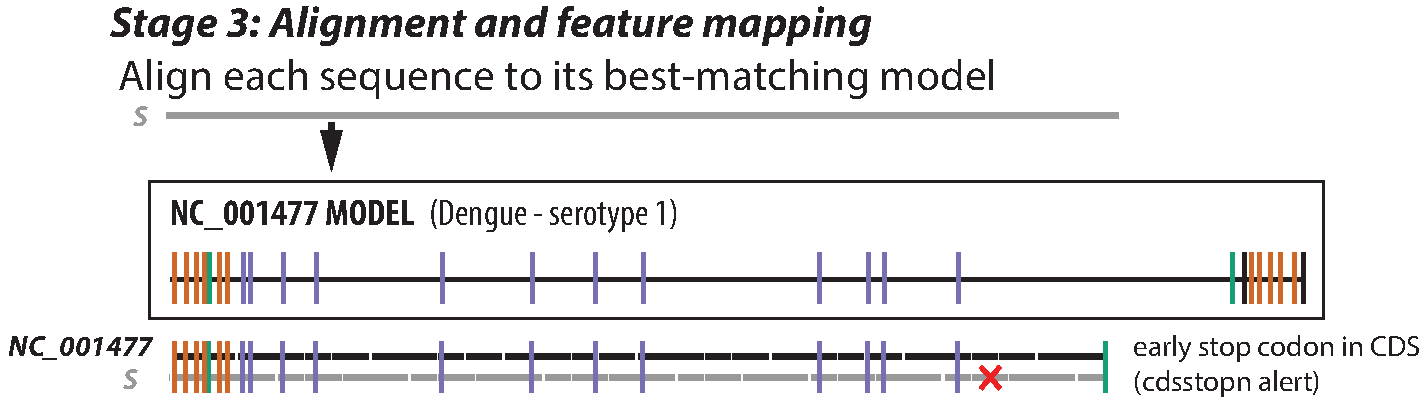
\includegraphics[width=10.5in]{figs/v-annotate-alignment-single-slide}

\end{center}
\vfill
\end{slide}
%%%%%%%%%%%%%%%%%%%%%%%%%%%%%%%%%%%%%%%%%%%%%%%%%%%%%%%%%%%%%%%%%%%%%%
\begin{slide}
\begin{center}

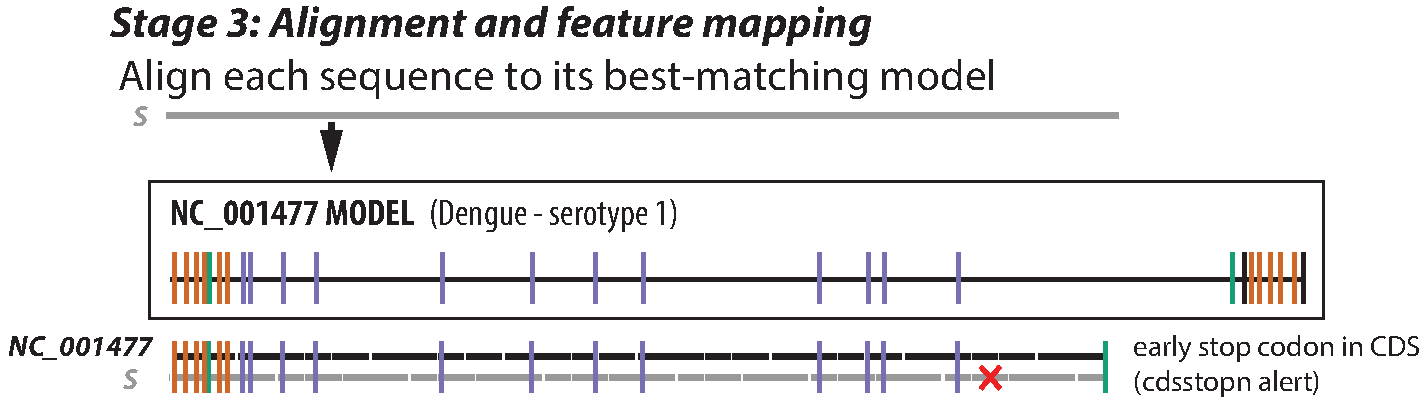
\includegraphics[width=10.5in]{figs/v-annotate-alignment-single-slide}
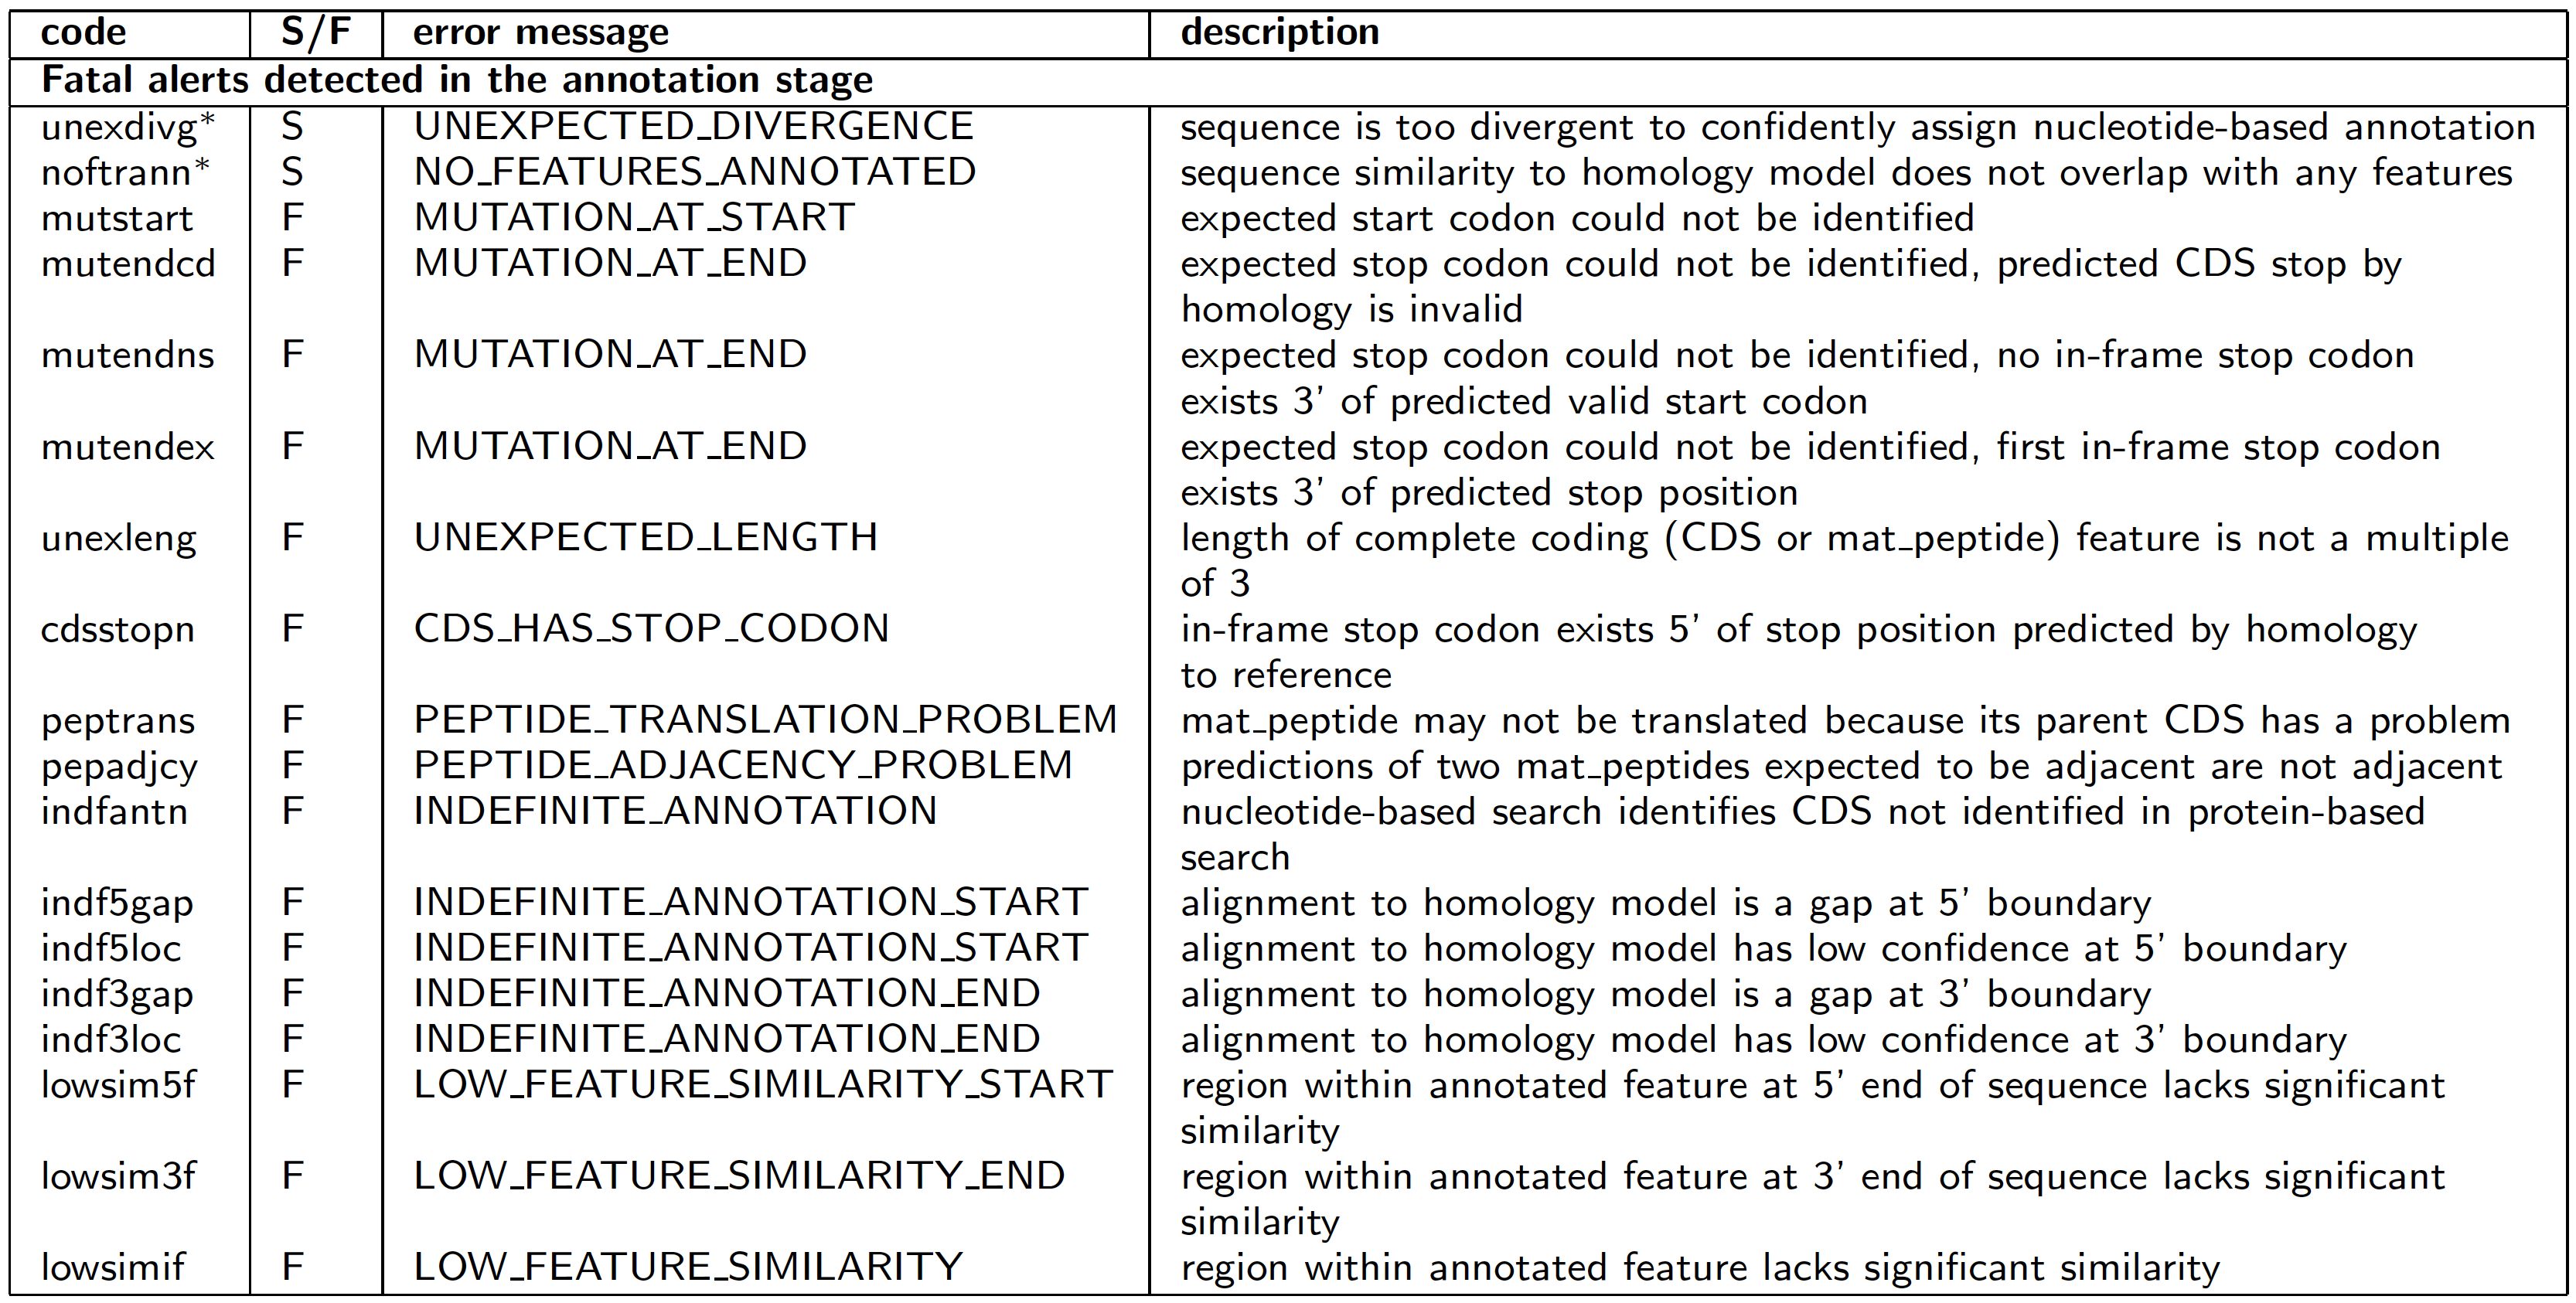
\includegraphics[width=10.5in]{figs/ss-alignment-alert-list}

\end{center}
\vfill
\end{slide}
%%%%%%%%%%%%%%%%%%%%%%%%%%%%%%%%%%%%%%%%%%%%%%%%%%%%%%%%%%%%%%%%%%%%%%
\begin{slide}
\begin{center}
\normalsize{\textbf{VADR used for Norovirus and Dengue virus sequences since 2018}}

\scriptsize
\begin{tabular}{r|r|r}
                                                  &Norovirus      &Dengue virus   \\ \hline
length                                            &7.6Kb         &10.7Kb        \\
\# seqs                                           &44,936          &113,211         \\
\% seqs full length                               &5.1\%          &8.4\%          \\
\% Ns                                             &0.5\%          &0.2\%          \\
\% seqs with stretch of $>=50$ Ns                 &1.0\%          &0.4\%          \\
average \% identity                               &81.6\%         &94.4\%         \\ \hline
\multicolumn{3}{l}{} \\ 
\multicolumn{3}{l}{\textbf{VADR v1.0 performance}} \\ \hline
seconds per sequence                   &42.4           &92.6           \\
required RAM                           &8Gb            &8Gb            \\
total running time, CPU days           &1.1            &10.2           \\
\end{tabular}
\end{center}

\vfill
\end{slide}
%%%%%%%%%%%%%%%%%%%%%%%%%%%%%%%%%%%%%%%%%%%%%%%%%%%%%%%%%%%%%%%%%%%%%%
\begin{slide}
\begin{center}
\normalsize{\textbf{SARS-CoV-2 sequence submissions have increased since early 2020}}
\end{center}

\tiny
\begin{center}
\begin{tabular}{llrr}
          &          &\#new     &\#cumulative\\
month     &year      &seqs      &seqs      \\ \hline
Jan       & 2020     &32        &32        \\ 
Feb       & 2020     &58        &90        \\ 
Mar       & 2020     &332       &422       \\ 
Apr       & 2020     &1541      &1963      \\ 
May       & 2020     &2974      &4937      \\ 
Jun       & 2020     &3394      &8331      \\ 
Jul       & 2020     &3604      &11,935    \\ 
Aug       & 2020     &3818      &15,753    \\ 
Sep       & 2020     &6731      &22,484    \\ 
Oct       & 2020     &11,939    &34,423    \\ 
Nov       & 2020     &4274      &38,697    \\ 
Dec       & 2020     &4530      &43,227    \\ 
& & & \\
Jan       & 2021     &8775      &52,002    \\ 
Feb       & 2021     &26,078    &78,080    \\ 
Mar       & 2021     &42,607    &120,687   \\ 
Apr       & 2021     &97,095    &217,782   \\ 
May       & 2021     &104,729   &322,511   \\ 
Jun       & 2021     &46,187    &368,698   \\ 
Jul       & 2021     &43,336    &412,034   \\ 
Aug       & 2021     &141,958   &553,992   \\ 
Sep       & 2021     &267,562   &821,554   \\ 
Oct       & 2021     &239,296   &1,060,850 \\ 
Nov       & 2021     &267,270   &1,328,120 \\ 
Dec       & 2021     &288,771   &1,616,891 \\ 
& & & \\
Jan       & 2022     &258,522   &1,875,413 \\ 
Feb       & 2022     &230,185   &2,105,598 \\ 
\end{tabular}
\end{center}

\vfill
\end{slide}
%%%%%%%%%%%%%%%%%%%%%%%%%%%%%%%%%%%%%%%%%%%%%%%%%%%%%%%%%%%%%%%%%%%%%%
\begin{slide}
\begin{center}
\normalsize{\textbf{SARS-CoV-2 sequences differ from Norovirus and Dengue virus \\ in several ways that impact VADR processing}}

\scriptsize
\begin{tabular}{r|r|r|r}
                                                  &Norovirus      &Dengue virus   &\textcolor{red}{SARS-CoV-2}      \\ \hline
length                                            &7.6Kb         &10.7Kb       &\textcolor{red}{29.9Kb}        \\
\# seqs                                           &44,936          &113,211         &\textcolor{red}{1,616,891}        \\
\% seqs full length                               &5.1\%          &8.4\%          &\textcolor{red}{99.7\%}         \\
\% Ns                                             &0.5\%          &0.2\%          &\textcolor{red}{1.4\%}          \\
\% seqs with stretch of $>=50$ Ns                 &1.0\%          &0.4\%          &\textcolor{red}{38.7\%}         \\
average \% identity                               &81.6\% &94.4\%         &\textcolor{red}{99.4\%}         \\ \hline
\multicolumn{4}{l}{} \\ 
\multicolumn{4}{l}{\textbf{VADR v1.0 performance}} \\ \hline
seconds per sequence                   &42.4           &92.6           &\textcolor{red}{331.8}          \\
required RAM                           &8Gb            &8Gb            &\textcolor{red}{64Gb}           \\
total running time, CPU days           &1.1            &10.2           &\textcolor{red}{6187.6}         \\
\end{tabular}
\end{center}

\vfill
\end{slide}
%%%%%%%%%%%%%%%%%%%%%%%%%%%%%%%%%%%%%%%%%%%%%%%%%%%%%%%%%%%%%%%%%%%%%%
\begin{slide}
\begin{center}
\normalsize{\textbf{Replacing Ns with expected nucleotides allows \\ many 'good' sequences to pass}}

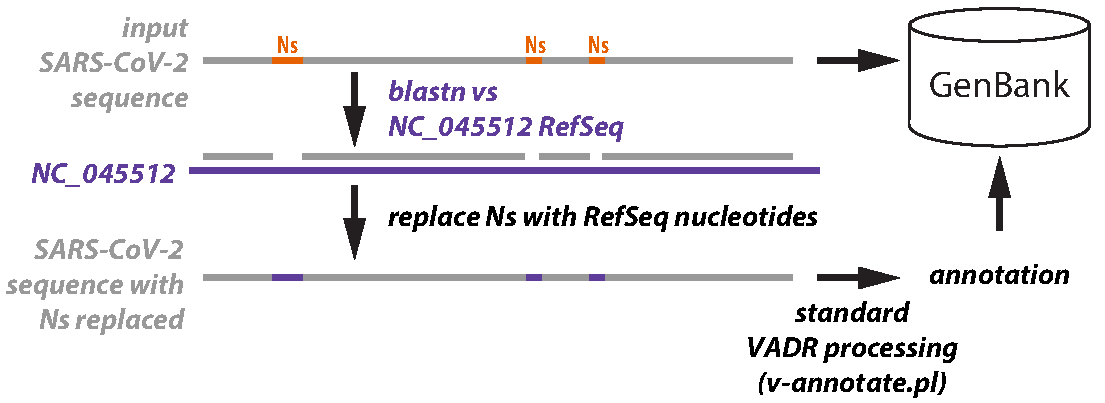
\includegraphics[width=10.25in]{figs/vadr-r-option}
\end{center}

\vfill
\end{slide}
%%%%%%%%%%%%%%%%%%%%%%%%%%%%%%%%%%%%%%%%%%%%%%%%%%%%%%%%%%%%%%%%%%%%%%
\begin{slide}
\begin{center}
\normalsize{\textbf{Seeded alignment using blastn makes alignment stage faster}}

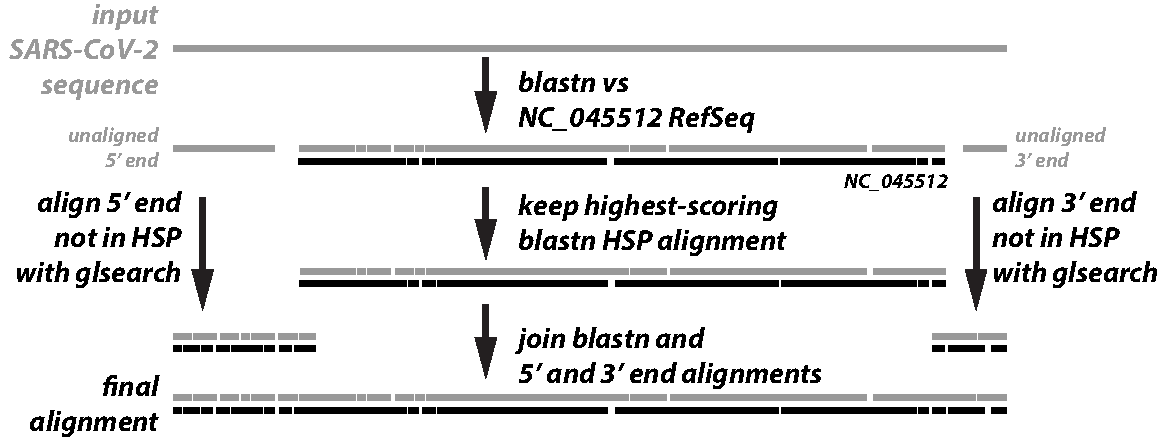
\includegraphics[width=10.25in]{figs/vadr-s-option}
\end{center}

\vfill
\end{slide}
%%%%%%%%%%%%%%%%%%%%%%%%%%%%%%%%%%%%%%%%%%%%%%%%%%%%%%%%%%%%%%%%%%%%%%
\begin{slide}
\begin{center}
\textbf{Using glsearch instead of cmalign reduces memory requirement}
\end{center}

\begin{itemize}
\item lower memory requirement (2Gb max) allows for multi-threading
%  \item input file is split into chunks
%    \begin{itemize}
%    \item each chunk processed independently in parallel on one of 8 CPUs
%    \item further reduces memory requirement for large input files \\ (dependent on chunk size
%      instead of input file size)
%    \end{itemize}
\end{itemize}

\begin{center}
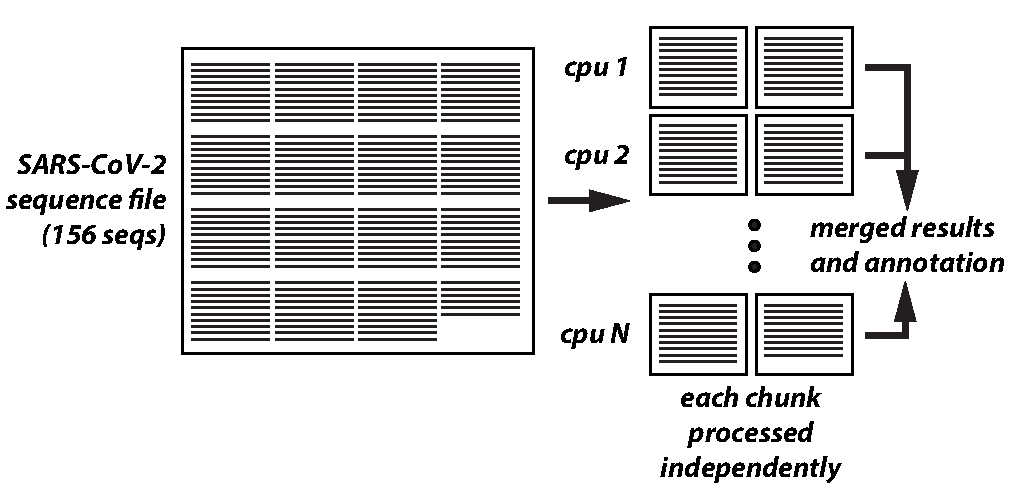
\includegraphics[width=10.5in]{figs/vadr-1p2-multithreading}
\end{center}
  
\vfill
\end{slide}
%%%%%%%%%%%%%%%%%%%%%%%%%%%%%%%%%%%%%%%%%%%%%%%%%%%%%%%%%%%%%%%%%%%%%%
\begin{slide}
\begin{center}
\normalsize{\textbf{VADR is now 1000-fold faster in practice for SARS-CoV-2 processing}}

\scriptsize
\begin{tabular}{lrrrrrrrr}
            &seeded      &N           &            &            &            &secs        &hours       &speedup     \\ 
VADR        &align-      &replace-    &            &\#          &required    &per         &per 100K    &vs          \\ 
version     &ment?       &ment?       &glsearch?   &cpus        &RAM         &seq         &seqs        &v1.0        \\ 
\hline
& & & & & & & & \\
v1.0        &$-$         &$-$         &$-$         &1           &64 Gb       &329.91      &9164.3      &-           \\
\end{tabular}
\end{center}

\vfill
\end{slide}
%%%%%%%%%%%%%%%%%%%%%%%%%%%%%%%%%%%%%%%%%%%%%%%%%%%%%%%%%%%%%%%%%%%%%%
\begin{slide}
\begin{center}
\normalsize{\textbf{VADR is now 1000-fold faster in practice for SARS-CoV-2 processing}}

\scriptsize
\begin{tabular}{lrrrrrrrr}
            &seeded      &N           &            &            &            &secs        &hours       &speedup     \\ 
VADR        &align-      &replace-    &            &\#          &required    &per         &per 100K    &vs          \\ 
version     &ment?       &ment?       &glsearch?   &cpus        &RAM         &seq         &seqs        &v1.0        \\ 
\hline
& & & & & & & & \\
v1.0         &$-$         &$-$         &$-$         &1           &64 Gb       &329.91      &9164.3      &-           \\
%1.1         &$+$         &$+$         &$-$         &1           &64 Gb       &49.35       &1370.7      &6.7         \\
& & & & & & & & \\
v1.4.1       &$+$         &$+$         &$+$         &1           &2 Gb        &2.51        &69.8        &131.4       \\
\end{tabular}
\end{center}

\vfill
\end{slide}
%%%%%%%%%%%%%%%%%%%%%%%%%%%%%%%%%%%%%%%%%%%%%%%%%%%%%%%%%%%%%%%%%%%%%%
\begin{slide}
\begin{center}
\normalsize{\textbf{VADR is now 1000-fold faster in practice for SARS-CoV-2 processing}}

\scriptsize
\begin{tabular}{lrrrrrrrr}
            &seeded      &N           &            &            &            &secs        &hours       &speedup     \\ 
VADR        &align-      &replace-    &            &\#          &required    &per         &per 100K    &vs          \\ 
version     &ment?       &ment?       &glsearch?   &cpus        &RAM         &seq         &seqs        &v1.0        \\ 
\hline
& & & & & & & & \\
v1.0         &$-$         &$-$         &$-$         &1           &64 Gb       &329.91      &9164.3      &-           \\
%v1.1         &$+$         &$+$         &$-$         &1           &64 Gb       &49.35       &1370.7      &6.7         \\
& & & & & & & & \\
v1.4.1       &$+$         &$+$         &$+$         &1           &2 Gb        &2.51        &69.8        &131.4       \\
& & & & & & & & \\
%v1.4.1       &$+$         &$+$         &$+$         &2           &4 Gb        &1.49        &41.5        &220.8       \\
%& & & & & & & & \\
%v1.4.1       &$+$         &$+$         &$+$         &4           &8 Gb        &0.65        &18.0        &509.9       \\
%& & & & & & & & \\
\textbf{v1.4.1}&\textbf{$+$}&\textbf{$+$}&\textbf{$+$}&\textbf{8}  &\textbf{16 Gb}&\textbf{0.33}&\textbf{9.3}&\textbf{986.8}\\
& & & & & & & & \\
%v1.4.1       &$+$         &$+$         &$+$         &16          &32 Gb       &0.23        &6.5         &1417.9      \\
%& & & & & & & & \\
v1.4.1       &$+$         &$+$         &$+$         &32          &64 Gb       &0.13        &3.7         &2462.2      \\
\end{tabular}
\end{center}

\vfill
\end{slide}
%%%%%%%%%%%%%%%%%%%%%%%%%%%%%%%%%%%%%%%%%%%%%%%%%%%%%%%%%%%%%%%%%%%%%%
\begin{slide}
\begin{center}
\normalsize{\textbf{VADR is now fast enough to handle \\ hundreds of thousands of sequences per month}}
\end{center}

\tiny
\begin{center}
\begin{tabular}{llrr}
          &          &\#new     &\#cumulative\\
month     &year      &seqs      &seqs      \\ \hline
Jan       & 2020     &32        &32        \\ 
Feb       & 2020     &58        &90        \\ 
Mar       & 2020     &332       &422       \\ 
Apr       & 2020     &1541      &1963      \\ 
May       & 2020     &2974      &4937      \\ 
Jun       & 2020     &3394      &8331      \\ 
Jul       & 2020     &3604      &11,935    \\ 
Aug       & 2020     &3818      &15,753    \\ 
Sep       & 2020     &6731      &22,484    \\ 
Oct       & 2020     &11,939    &34,423    \\ 
Nov       & 2020     &4274      &38,697    \\ 
Dec       & 2020     &4530      &43,227    \\ 
& & & \\
Jan       & 2021     &8775      &52,002    \\ 
Feb       & 2021     &26,078    &78,080    \\ 
Mar       & 2021     &42,607    &120,687   \\ 
Apr       & 2021     &97,095    &217,782   \\ 
May       & 2021     &104,729   &322,511   \\ 
Jun       & 2021     &46,187    &368,698   \\ 
Jul       & 2021     &43,336    &412,034   \\ 
Aug       & 2021     &141,958   &553,992   \\ 
Sep       & 2021     &267,562   &821,554   \\ 
Oct       & 2021     &239,296   &1,060,850 \\ 
Nov       & 2021     &267,270   &1,328,120 \\ 
Dec       & 2021     &288,771   &1,616,891 \\ 
& & & \\
Jan       & 2022     &258,522   &1,875,413 \\ 
Feb       & 2022     &230,185   &2,105,598 \\ 
\end{tabular}
\end{center}

\vfill
\end{slide}
%%%%%%%%%%%%%%%%%%%%%%%%%%%%%%%%%%%%%%%%%%%%%%%%%%%%%%%%%%%%%%%%%%%%%%
\begin{slide}
\begin{center}
\textbf{Besides getting faster, VADR has changed in other ways \\ (work with Linda Yankie and Vince Calhoun and GenBank team)}

\begin{itemize}
\item 14 releases since March 2020
\item 3 additional models (all eventually dropped):
  \begin{itemize}
  \item B.1.1.7 (alpha)
  \item B.1.525
  \item 28254-deletion
  \end{itemize}
\item allow some alerts for non-essential ORFs without failing sequence \\ (they become a \texttt{misc\_feature} instead)
\end{itemize}

\end{center}

\vfill
\end{slide}
%%%%%%%%%%%%%%%%%%%%%%%%%%%%%%%%%%%%%%%%%%%%%%%%%%%%%%%%%%%%%%%%%%%%%%
\begin{slide}

\large
\begin{center}
\large{\textbf{Acknowledgements}} \\

\normalsize
\vspace{0.75in}

\small
\begin{tabular}{l|l|l}
%                  & \\ \hline
%                  & \\
\textbf{NCBI - viral annotation} & \textbf{NCBI - leadership} &  \textbf{Software developers} \\
Alejandro Sch\"{a}ffer (now NCI) & David Landsman             & Sean Eddy (HMMER/Infernal/Easel)\\
                                 & Kim Pruitt                 & Travis Wheeler (HMMER)\\
Linda Yankie                     & Steve Sherry               & Tom Madden and BLAST team \\
Vincent Calhoun                  & Jim Ostell                 & William Pearson (FASTA/glsearch) \\
Sergiy Gotvyanskyy               & David Lipman               & Michael Farrar (HMMER/glsearch) \\
Susan Schafer                    &                            & \\
Ilene Mizrachi                   & \textbf{NLM - leadership}  & \\
Colleen Bollin                   & Patti Brennan              & \\
Beverly Underwood                & Jerry Sheehan              & \\
Vasuki Gobu                      & Valerie Florance           & \\
Alex Kotliarov                   & & \\
& & \\
Rodney Brister                   & & \\
Eneida Hatcher                   & & \\
& & \\
Lara Shonkwiler                  & & \\
Sophia Hu                        & & \\
& & \\
Wratko Hlavina                   & & \\
Eyal Mozes                       & & \\
Ron Patterson                    & & \\
Sumit Saluja                     & & \\ 
\end{tabular}


\includegraphics[width=2.5in]{figs/NIH_NLM_ABRV_2C_4-white}

\includegraphics[width=2.5in]{figs/ncbi-logo}

\end{center}

\vfill
\end{slide}
%%%%%%%%%%%%%%%%%%%%%%%%%%%%%%%%%%%%%%%%%%%%%%%%%%%%%%%%%%%%%%%%%%%%%%
\end{document}
%%%%%%%%%%%%%%%%%%%%%%%%%%%%%%%%%%%%%%%%%%%%%%%%%%%%%%%%%%%%%%%%%%%%%%

